\chapter{REVISÃO DE LITERATURA}
\label{chap:fundamentacaoTeorica}

Neste capítulo, são apresentados alguns conceitos e termos utilizados no decorrer do trabalho. 
Os conceitos apresentados tem relação com a construção do sistema. São apresentadas as 
técnicas, arquiteturas e algoritmos disponíveis para solução do problema, assim como as utilizadas no 
desenvolvimento da solução.

As primeiras seções do capítulo abordam os padrões e protocolos disponíveis na literatura que são 
utilizados na construção de \textit{webservices}.  Esses padrões e protocolos 
são conhecidos por facilitar e flexibilizar a integração de sistemas. 
Entre eles destacam-se o \textit{Service Oriented Architecture} (SOA), que é
uma arquitetura que trata os serviços como componentes e visa utilizar 
esses componentes para resolver problemas de negócios complexos através de composição
de serviços. \textit{Representational State Transfer} (REST), que é um estilo arquitetural 
que pode ser utilizado, ou não, para a criação de serviços SOA. O \textit{Simple Object Access Protocol}
(SOAP), que é um protocolo que muitas vezes é comparado ao REST por também servir
para a criação de serviços SOA.

Além disso, nas seções posteriores, o capítulo também apresenta algoritmos que ajudam a 
resolver o problema da seleção de host para migração de VM através de otimização multi-objetivo (MOO). 
Existem vários algoritmos que podem ser utilizados para a resolução desse tipo de problema. 
Neste trabalho, são abordados os algoritmos genéticos (GAs), que fazem parte de um grupo 
maior de algoritmos, chamado algoritmos evolucionários (EAs). 
O conceito de EA também será abordado neste capítulo.

Nas primeiras quatro seções, as ferramentas apresentadas 
estão relacionadas em como é feita a comunicação e disponibilização do serviço. 
E as outras seções estão relacionados ao funcionamento interno, em como solucionar
a seleção dos melhores hosts.

\section{SERVICE ORIENTED ARCHITECTURE (SOA)}
O desenvolvimento de software para um ambiente corporativo é uma tarefa complexa. 
Conforme Brown \cite{brown}, no decorrer dos anos, a comunidade de desenvolvimento de software se 
dedicou em desenvolver novas abordagens, processos e ferramentas para a construção de softwares de 
grande escala. 

Brown considera que uma maneira de descrever um sistema de software é como sendo um composto de 
uma coleção de serviços. Cada serviço, provém um conjunto de funcionalidades bem definidas. 
As funcionalidades do serviço sendo bem definidas tornam possível a construção de serviços 
compostos, ou seja, uma funcionalidade que faça a utilização de outras funcionalidades ou serviços. 
Esta modularização e coordenação de serviços e funcionalidades caracteriza uma 
Service Oriented Architecture (SOA).

Segundo \cite{valipour}, SOA pode ser definido como um design de software utilizado para 
conectar negócios e recursos computacionais sob demanda, e isso possibilita os usuários 
do serviço (podendo ser outros serviços ou usuários finais) a alcançarem seus objetivos. 

Existem diversas maneiras de implementar uma aplicação baseada em SOA, o importante é que 
sua interface seja bem definida com as operações que podem ser realizadas. 
Uma das grandes vantagens do SOA, é a facilidade que ele provém na integração de sistemas. 
Segundo \cite{valipour}, com as operações bem definidas e disponíveis, o consumidor do SOA, 
pode se preocupar somente com o que determinado serviço faz e não como é implementado.

As principais características de um software feito utilizando SOA são que ele é auto contido e 
modular, interoperável, fracamente acoplado, passível de composição e possui transparência de localização. 
Como SOA não limita a estratégia utilizada para o desenvolvimento do mesmo, pode-se utilizar qualquer 
técnica para implementá-lo. No ambiente corporativo, os serviços comumente são implementados 
utilizando web services SOAP, REST ou chamadas RPCs.

\subsection{Enterprise Service Bus (ESB)}

Para obter essa flexibilidade na construção dos serviços, é comum que com SOA se
utilize uma camada que recebe a chamada dos serviços e encaminha para o serviço correto,
ela faz isso através de um enfileiramento de mensagens.
Essa camada, além de ter responsabilidade enfileirar as mensagens enviadas aos serviços,
também pode fazer a tradução da comunicação, caso um serviço trabalhe somente com SOAP e outro somente
com REST.

A arquitetura utilizando SOA fica semelhante a da Figura \ref{fig:soaesb}.

\begin{figure}[!htb]
  \centering
  \caption{SOA com ESB}
  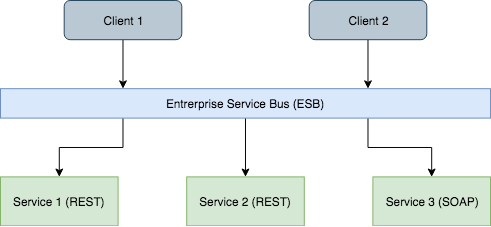
\includegraphics[width=1\textwidth]{./dados/figuras/SOA.png}
  \label{fig:soaesb}
\end{figure}

\section{REPRESENTATIONAL STATE TRANSFER (REST)}
REST foi formalizado por Fielding \cite{fielding} em sua tese de doutorado, onde ele tem por 
objetivo apresentar uma arquitetura para criação de sistemas network-based. 
Na tese, REST é definido como um estilo arquitetural. Fielding também define seis diretivas que 
devem ser respeitadas na criação de um software que é implementado utilizando este estilo arquitetural. 
As diretivas são maneiras de implementar a API para simplificar o uso e melhorar a 
arquitetura da API que está sendo construída. 

A comunicação no REST, é feita via \textit{Hypertext Trasfer Protocol} (HTTP). Desta meneira
a comunicação cliente-servidor é feita utilizando as funcionalidades que o protocolo suporta,
como: a utilização de cabeçalhos, \textit{query-strings}, \textit{Universal Resource Identifiers}(URIs),
entre outros recursos do protocolo.

\begin{figure}[!htb]
  \centering
  \caption{REST sobre HTTP simples}
  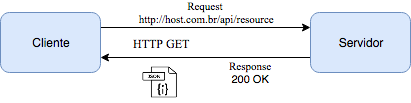
\includegraphics[width=1\textwidth]{./dados/figuras/rest-1.png}
  \label{fig:rest1}
\end{figure}

Neste capítulo são apresentadas as seis diretivas que são definidas por Fielding
que um sistema deve atender quando REST é utilizado e a maneira de utilização dos
verbos HTTP no padrão arquitetural. 

As diretivas, podem ser atendidas em sua totalidade
ou não, isso depede do nível de maturidade da API. Uma API que não atende todas as diretivas 
não está deixando de utilizar REST, apenas o utiliza com um nível de maturidade
menor. As seis diretivas do REST são:

\begin{enumerate}
  \item Interface uniforme
  \item \textit{Stateless}
  \item Cacheável
  \item Cliente-servidor
  \item Sistema em camadas
  \item Código por demanda (Opcional)
\end{enumerate}

\subsection{Interface Uniforme}

Fielding \cite{fielding} destaca que uma das características centrais do REST, e o que difere ele 
de outros estilos arquiteturais, é a utilização de uma interface uniforme entre os componentes. 
Esta interface uniforme define a forma com que o cliente e o servidor se comunicam. Segundo \cite{todd}
isto desacopla e simplifica a arquitetura.

Segundo \cite{todd} além disso, essa interface, é uniforme quando segue as seguintes características:

\begin{enumerate}
  \item Baseada em recurso
  \item Manipula os recursos através de representações
  \item Possui mensagens autodescritivas
  \item \textit{Hypermedia as the Engine of Application State} (HATEOAS)
\end{enumerate}

Ser \textbf{baseada em recursos}, significa que a interface deve separar seus
recursos através de URIs. 
Cada recurso possui alguma URI que serve como \textit{endpoint} para interação com o usuário. 
Essa URI é utilizada para fazer a \textbf{manipulação dos recursos utilizando representações}.
As representações de um recursos podem ter diversos formatos, como por exemplo 
\textit{JavaScript Object Notation} (JSON) ou \textit{eXtensible Markup Language}(XML).

\textbf{Mensagens autodescritivas} significa que na requisição feita pelo cliente para
o servidor, devem ser incluidas informações sobre o que deve ser feito com o recurso
que se está utilizando. Por exemplo, deve ser incluido o formato que está sendo feita a
comunicação (XML, JSON), o que está querendo modificar naquele recurso (atualizar, deletar, etc.).
Além dessas informações, que são enviadas pelo cliente, as mensagens de resposta também devem 
ser autodescritivas, contendo informações sobre a resposta, por exemplo, se o recurso pode ser
cacheado e por quanto tempo.

Segundo \cite{todd} \textbf{HATEOAS} significa clientes entregar estado via conteúdo no corpo
da mensagem, \textit{query-strings}, cabeçalhos e URIs. E o servidor retornar estados
através de \textit{status-codes}, conteúdo no corpo da mensagem e meta-informações através
de cabeçalhos. Seguindo essas regras, a comunicação é considerada comunicação via \textbf{hyperteto}.
Além disso, também significa enviar a relação entre recursos quando necessário. Isso pode
ser feito através de links contidos nos corpos da mensagem ou cabeçalhos da requisição.

\begin{figure}[!htb]
  \centering
  \caption{Recursos REST}
  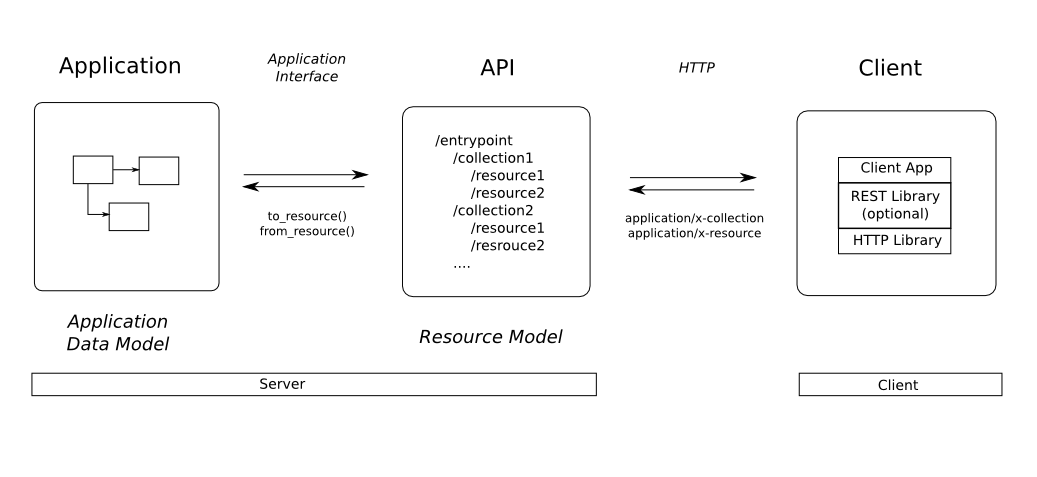
\includegraphics[width=1\textwidth]{./dados/figuras/rest-2.png}
  \label{fig:rest2}
\end{figure}

\subsection{Cliente-servidor}

REST é implementado utilizando o modelo de comunicação cliente-servidor. 
Isso ajuda com a separação de responsabilidades, e permite que uma portabilidade 
de clientes do serviço implementado. O REST permite uma reutilização do serviço. 
Do ponto de vista de arquitetura de software, isto é muito importante, pois permite 
que componentes fiquem bem modularizados.

\subsection{Stateless}

No REST, é necessário que a aplicação seja \textit{Stateless}, ou seja, as requisições
devem ser autocontidas. Isso significa que as requisições de usuários devem conter todas
as informações necesárias para o servidor entender e processar a requisição. Não deve-se
assumir que o cliente da API utilize-a de uma forma específica para a requisição funcionar.

\subsection{Cacheável}

Essa é uma característica que faz com que aumente o desempenho da aplicação. Deve ser
possível fazer cache de informações. Isso faz com que gere menos comunicação entre
cliente e servidor. O \textit{cache} pode ser feito de maneira implicita (o cliente
define quando cachear) e de maneira explícita (o servidor indica que a requisição pode
ser cacheada).

\subsection{Sistemas em camadas}

Deve ser possível adicionar camadas(\textit{middlewares}) na utilização do REST.
Essas camadas podem ter diversas finalidades, como, por exemplo, aumento de performance
através de \textit{load-balance}, aumento de segurança (autenticação), entre outros.

\subsection{Código por demanda (Opcional)}

Esta restrição é opcional e pouco utilizada. Segundo \cite{todd} é uma maneira de
extender a funcionalidade através de envio de código para ser executado pelo cliente.
Esta restrição deve ser aplicada apenas quando não viole outras diretivas.

\subsection{Verbos HTTP}

Além dos itens citados nas seções anteriores, outra parte importante no REST,
para a uniformidade da interface, são os \textbf{verbos http}. Os verbos
HTTP representam a ação que o usuário da API está querendo tomar através da
requisição enviada. Isso é muito importante, pois atribuí um contexto para cada
tipo de requisição da API através do tipo do verbo utilizado.

\begin{table}[!htb]
    \centering
    \caption[Verbos HTTP]{Tabela de verbos HTTP
    \label{tab:verbos-http}}
    \begin{tabular}{rrrrr}
        \toprule
            Verbo & Descrição \\ 
        \midrule
            GET & busca/le informações na API \\
            POST & cria recursos na API \\
            PUT &  atualiza algum recurso \\
            DELETE  & deleta algum recurso ou alguns recursos \\
        \bottomrule
    \end{tabular}
\end{table}

\section{SIMPLE OBJECT ACCESS PROTOCOL (SOAP)}
SOAP é um protocolo de comunicação baseado em XML(eXtension Markup Language) que foi criado no final 
dos anos 90. Seu objetivo é fazer a comunicação entre o cliente e o servidor através de informações 
passadas através de um documento XML. O protocolo utiliza um \textit{schema} XML, que é uma 
maneira de descrever e validar o formato os dados das requisições e respostas. 
Esse \textit{schema} é utilizado pelo cliente e pelo servidor para saber como interpretar 
a resposta, no caso de recebimento de mensagem, e formatar a requisição, no caso de envio.
Esse \textit{schema} é chamado de WSDL (Web Services Description Language).

O objetivo do SOAP, é expor regras de negócio de aplicação através de serviços. 
Por esse motivo, o SOAP é uma opção comumente utilizada na construção de aplicações SOA. 
Outra característica do SOAP, é que ele não precisa ser implementado sobre um protocolo de 
transporte específico, e na maioria das vezes é utilizado HTTP, porém é possível implementá-lo
utilizando outros protocolos. Além do SOAP permitir utilizar outro protocolo, 
ele não restringe a implementação em alguma linguagem de programação específica, ou seja,
é possível implementá-lo em qualquer linguagem de programação.

O SOAP é comparado ao REST, pois os dois podem ser utilizados para um objetivo 
semelhante, porém, os dois tem um foco diferente, onde o SOAP tem como objetivo expor regras de negócio 
como serviço, e o REST visa representar um determinado estado e manipulá-lo através de operações 
bem definidas.

Segundo \cite{lecheta} como o SOAP é um grande XML, no contexto dos webservices, ele começou
a parder espaço para o REST, o qual é mais simples 
e permite enviar informações em formatos mais leves, como o JSON por exemplo. 
Isso é uma grande vantagem, principalmente por ser um problema
que tem o potencial de ter quantidade de dados trafegando em larga escala.

Uma comparação do SOAP com o rest, pode ser observado na Tabela \ref{tab:rest-vs-soap}

\begin{table}[!htb]
    \centering
    \caption[REST vs. SOAP]{Tabela comparativa REST vs. SOAP
    \label{tab:rest-vs-soap}}
    \begin{tabular}{|m{3cm}|m{6cm}|m{6cm}|}
        \toprule
            Comparação & \textbf{SOAP} & \textbf{REST} \\
        \midrule
            \textbf{Design} & Protocolo bem definido com regras para seguir & Estilo arquitetural com diretrizes e recomendações\\
            \textbf{Formato de Mensagens} & Somente \textbf{XML} & Vários formatos, como \textbf{XML}, \textbf{JSON}, \textbf{HTML}, etc. \\
            \textbf{Abordagem} & Guiado por funções, mais ligadas ao negócio, por exemplo (getUser, proccessOrder) & Guiado por dados, os dados ficam disponíveis através de recursos, por exemplo (users) \\
            \textbf{Protocolo de comunicação} & Qualquer protocolo (UDP, HTTP, TCP/IP) & Apenas HTTP \\
            \textbf{Cache} & Não é possível fazer cache & É possível fazer cache \\
        \bottomrule
    \end{tabular}
\end{table}

\section{ALGORITMOS GENÉTICOS (GA)}
Algoritmos genéticos (GAs) são uma classe de algoritmos que se baseam
na evolução natural de Darwin. Esse processo envolve criar uma população,
selecionar os indivíduos mais aptos através de uma função objetivo,
aplicar mutação e \textit{crossover} na população. 
Esse processo resulta em gerações (novas populações)
mais adequadas em relação ao objetivo que está sendo
avaliado na fase de seleção, assim como ocorre na teoria da 
seleção natural, os mais "adequados" sobrevivem. O processo evolutivo 
(os passos anteriores para geração de novas populações)
continua até que haja um critério de parada. Este processo é
ilustrado no fluxograma da Figura \ref{fig:gaalgorithm}.

De maneira geral, o GA utiliza a função objetivo (OF) para
a seleção, ou seja, escolha dos mais adequados, 
utiliza o \textit{crossover} para a convergência das soluções para melhores soluções,
e a mutação como operador de diversidade. Estes operadores são importante para
obter tipos diferentes de soluções, inicialmente inexplorados pelo algoritmo.

\begin{figure}[!htb]
  \centering
  \caption{Exemplo GA}
  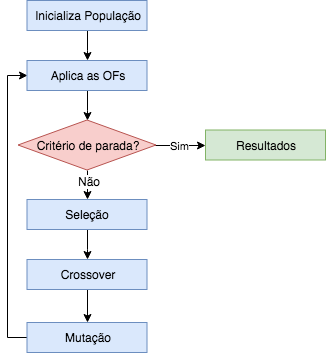
\includegraphics[width=0.65\textwidth]{./dados/figuras/ga-algorithm.png}
  \label{fig:gaalgorithm}
\end{figure}

\subsection{Seleção}
Conforme \cite{ghosh}, o principal objetivo do operador de seleção é
manter as soluções boas e eliminar as ruins mantendo o tamanho da população
constante.

Existem vários tipos de operadores de seleção. Entre eles, os mais comuns são: 
\textbf{Tournament Selection}, \textbf{Proportionate Selection} e 
\textbf{Ranking Selection}. Cada tipo de operador de seleção utiliza uma estratégia diferente 
para fazer a seleção dos melhores indivíduos. O resultado da seleção 
feita por esse tipo de operador é chamada de \textit{mating pool}, que representam 
os indivíduos selecionados para a reprodução.

\subsection{\textit{Crossover}}
O operador de \textit{crossover} é responsável pelo processo onde dois cromossomos 
são cruzados. Segundo \cite{ghosh}, dois cromossomos são selecionados da \textit{mating pool}
e parte deles são misturados para que seja feita a criação de novos indivíduos. 
Nos GAs a quantidade de indivíduos que são escolhidos para o cruzamento, dependem da probabilidade
de crossover. Após o cruzamento, é gerada uma nova geração (\textit{offspring population}). 
Depois da fase de \textit{crossover}, o algoritmo segue para a mutação,
conforme a Figura \ref{fig:gaalgorithm} ilustra.

\subsection{Mutação}
A mutação é uma etapa que é responsável por manter a diversidade na população. Isso
é feito através da mudança do valor de genes de algum cromossomo da população. Geralmente, o operador
de mutação é utilizado com uma probabilidade baixa, pois caso contrário, seriam
geradas somente populações aleatórias. 

A mutação do gene é importante para que as gerações não tenham uma convergência para 
um único ponto. Tanto o crossover quanto a mutação, fazem com que o espaço de busca
de soluções ótimas, seja ampliado. Isso é importante para que nenhuma solução ótima
passe despercebido. Sem este operador de diversidade, as soluções podem convergir para
um ponto em que todas fiquem muito parecidas, o que não é interessante pois soluções
melhores podem estar localizadas em um ponto diferente da busca.

Segundo \cite{ghosh}, estes operadores genéticos do GA, podem ser usados para otimizar tanto
problemas mono-objetivo e também multi-objetivo. Neste trabalho, será utilizado
o algoritmo para um problema multi-objetivo, por esse motivo, a próxima seção aborda
este tipo de problema.

\section{OTIMIZAÇÃO MULTI-OBJETIVO (MOO)} 
Segundo \cite{ghosh} um problema de otimização multi-objetivo, como
o próprio nome sugere, possui N objetivos que devem ser otimizados. 
Na otimização multi-objetivo, existem duas variáveis importantes
para fazer a seleção dos indivíduos de uma população,
que são o espaço de busca (\textit{search space}) e o 
espaço dos objetivos (\textit{objective space}).

O espaço de busca é representado pelos valores das variávies dos 
indivíduos de uma população. Através desses valores, os indivíduos
são avaliados e possuem um valor correspondente no \textit{objective space}. 
Este valor é calculado através de seu \textit{fitness}, ou seja, representa
o quão apto aquele espaço de busca é em relação aos objetivos.

\begin{figure}[!htb]
  \centering
  \caption{Espaço de decisáo e espaço dos objetivos}
  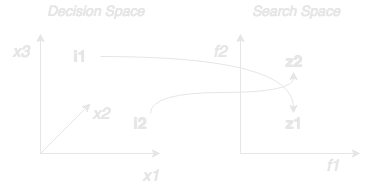
\includegraphics[width=0.9\textwidth]{./dados/figuras/searchspace-decisionspace.png}
  \label{fig:moospaces}
\end{figure}

\subsection{Dominância de pareto}
Após o mapeamento do espaço de busca e espaço de objetivos, é necessário
ter uma maneira de reconhecer os melhores indivíduos. Uma possível
estratégia para o reconhecimento dos melhores no contexto de MOO 
é a \textbf{Dominância de Pareto}.

Segundo \cite{ghosh}, problemas de MOO, as OFs são conflitantes por natureza, e 
por consequência, cada OF possui uma solução ótima. Para resolver este problema,
as OFs não devem ser consideradas individualmente na avaliação de um indivíduo.
Sendo assim, uma solução é dominada caso nenhum objetivo seja melhor do que
o qual está sendo comparado. Por exemplo:

\begin{enumerate}
  \item \textbf{s1 e s2} são duas soluções;
  \item \textbf{f1 e f2} são duas funções objetivo;
  \item \textbf{s1} domina \textbf{s2} se:
    \begin{enumerate}
      \item \textbf{f1 e f2} da \textbf{s1} tem melhores resultados que \textbf{s2}.
    \end{enumerate}
  \item \textbf{s1} tenha melhores resultados na OF \textbf{f1} e \textbf{s2} na OF \textbf{f2}
  ambas são consideradas não dominadas.
\end{enumerate}

O objetivo quando se está fazendo uma otimização multi-objetivo é buscar
a chamada \textbf{fronteira de pareto} ou \textit{pareto-front}. Onde, apenas
as soluções que não são dominadas por nenhuma outra solução fazem parte, ou seja,
são as melhores soluções para um problema levando em conta os múltiplos objetivos.

\begin{figure}[!htb]
  \centering
  \caption{Pareto-front}
  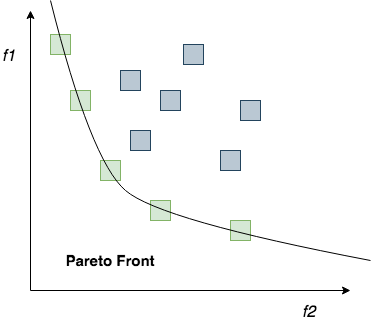
\includegraphics[width=0.6\textwidth]{./dados/figuras/pareto-front.png}
  \label{fig:paretofront}
\end{figure}

\section{TRABALHOS RELACIONADOS}
O OptVM busca oferecer um suporte para a migração de máquinas virtuais. Esse
suporte é oferecido através de um serviço que seleciona um subconjunto de hosts 
dos possíveis alvos de migração. Além disso, oferece uma maneira de restringir
a escolha dos hosts que não são elegiveis por questões relacionadas a negócio.

Esta seção apresenta alguns trabalhos relacionados ao problema que o OptVM está
se propondo a resolver.

\subsection{Migração de máquinas virtuais}
As nuvens computacionais são utilizadas pela maioria das empresas de software da atualidade. 
Por esse motivo, as maiores empresas do setor investem muito neste segmento, 
oferecendo vários tipos de serviços diferenciados para seus consumidores. 
Estas empresas concorrem em alguns aspectos, como: velocidade, preço, disponibilidade e etc. 
Para aumentar sua competitividade, é utilizada a virtualização.

Com a virtualização é possível alocar partes de um recurso físico para diferentes consumidores, 
fazendo com que um recurso físico se torne melhor utilizado. Isso deixa a alocação de recursos
muito mais flexível, e torna possível obter uma elasticidade nos serviços oferecidos. 

Uma dos objetivos de utilizar a virtualização é obter uma elasticidade dos recursos oferecidos.
Ou seja, é possível aumentar sua capacidade de processamento, armazenamento mesmo depois que o
já foi alocada uma VM para o usuário.
Isso permite que um consumidor do  serviço possa escolher o quanto precisa para executar as 
tarefas que deseja, assim como o provedor também consegue otimizar o uso de seus recursos. Porém,
existem casos onde uma máquina virtual não consegue aumentar seu consumo de recursos, por uma limitação
do host em que está alocada. Nestes casos, é necessário ser feito uma realocação de VM para outro 
host.

A realocação de uma VM pode ser feita a nível de nuvem, datacenter(DC) ou host.
Quando a realocação é feita em nível de DC ou nuvem, é muito provável que seja 
necessário migrar uma VM do local em que ela se encontra. 

Três momentos podem ser considerados os pontos principais a serem avaliados para uma migração, 
são eles:

\begin{enumerate}
\item A descoberta de uma necessidade de migração
\item Qual máquina virtual deve ser mgirada
\item Para onde deve ocorrer a migração
\end{enumerate}

As migrações das VMs são necessárias em ambientes que envolvem uma infraestruturas
grande, onde existem multiplos hosts, datacenters e nuvens. Por esse motivo, não é recomendado que 
um sistema ou serviço gerencie a infraestrutura inteira sozinho, pois sua escalabilidade 
poderia se tornar um gargalo. Isso faz com que sejam construidos diferentes serviços e aplicações 
que se integram e gerenciam a infraesturua.

O OptVM é uma alternativa para lidar com o terceiro momento da migração. 
Ajuda a escolher o destino da VM através de um \textit{webservice}. Isso 
remove uma das responsabilidades do serviço de gerencia da infraestrutura da
nuvem, diminuindo a possibilidade de um gargalo.
